%\section{Motion sensors as input devices}
\section{Gesture recognition devices}
Gesture recognition technology is a field that has gained much attention with the growth of the virtual reality field, 
and it's a very diverse one with roots in sensor technology, image processing and computer vision~\citep{Vafadar2014}. 
The first attempts at a commercial hand gesture recognition system were typically glove-based control interfaces, often called \textbf{\textit{data gloves}} 
and were gloves with sensors attached to it. As the image processing and computer vision technology wasn't mature yet, these \textbf{\textit{contact-based devices}} remained 
the primary gesture recognition technology, until the image processing-reliant \textbf{\textit{vision-based devices}} began to see some success in the 2000s~\citep{Premaratne2014}.
Another factor which made data gloves ideal was a very limited requirement for processing power, as any pre-processing were rarely done, 
and thus the systems could run optimally on the commodity 1980s and 1990s computers~\citep{Premaratne2014}.  

\begin{figure}%[h!] %[H]
	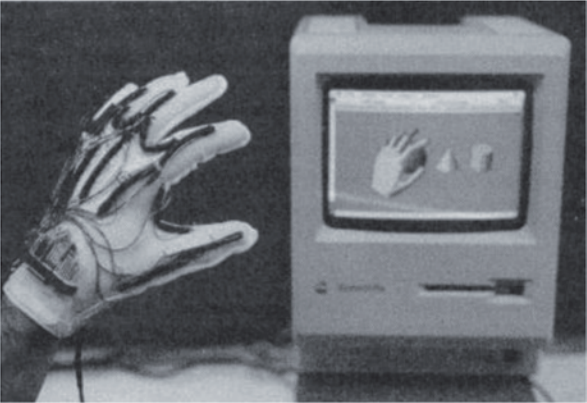
\includegraphics[width=\linewidth]{pictures/old_dataglove.png}
	\caption[The Z Glove]{The Z Glove, developed by Zimmerman in 1982. Picture from \citet{Premaratne2014}}
	\label{fig:old_dataglove}
\end{figure} 

Today, both contact-based and vision-based devices are utilized for gesture recognition purposes. 

\paragraph{Contact-based devices} are usually wearable objects, such as gloves or armbands, 
which register the user's kinetic movement through sensors and attempt to mirror it in the virtual world. 
Some notable products making use of this technology include the Nintendo Wii remote controller and the Myo armband (see figure \ref{fig:myo}). 

\begin{figure}%[h!] %[H]
	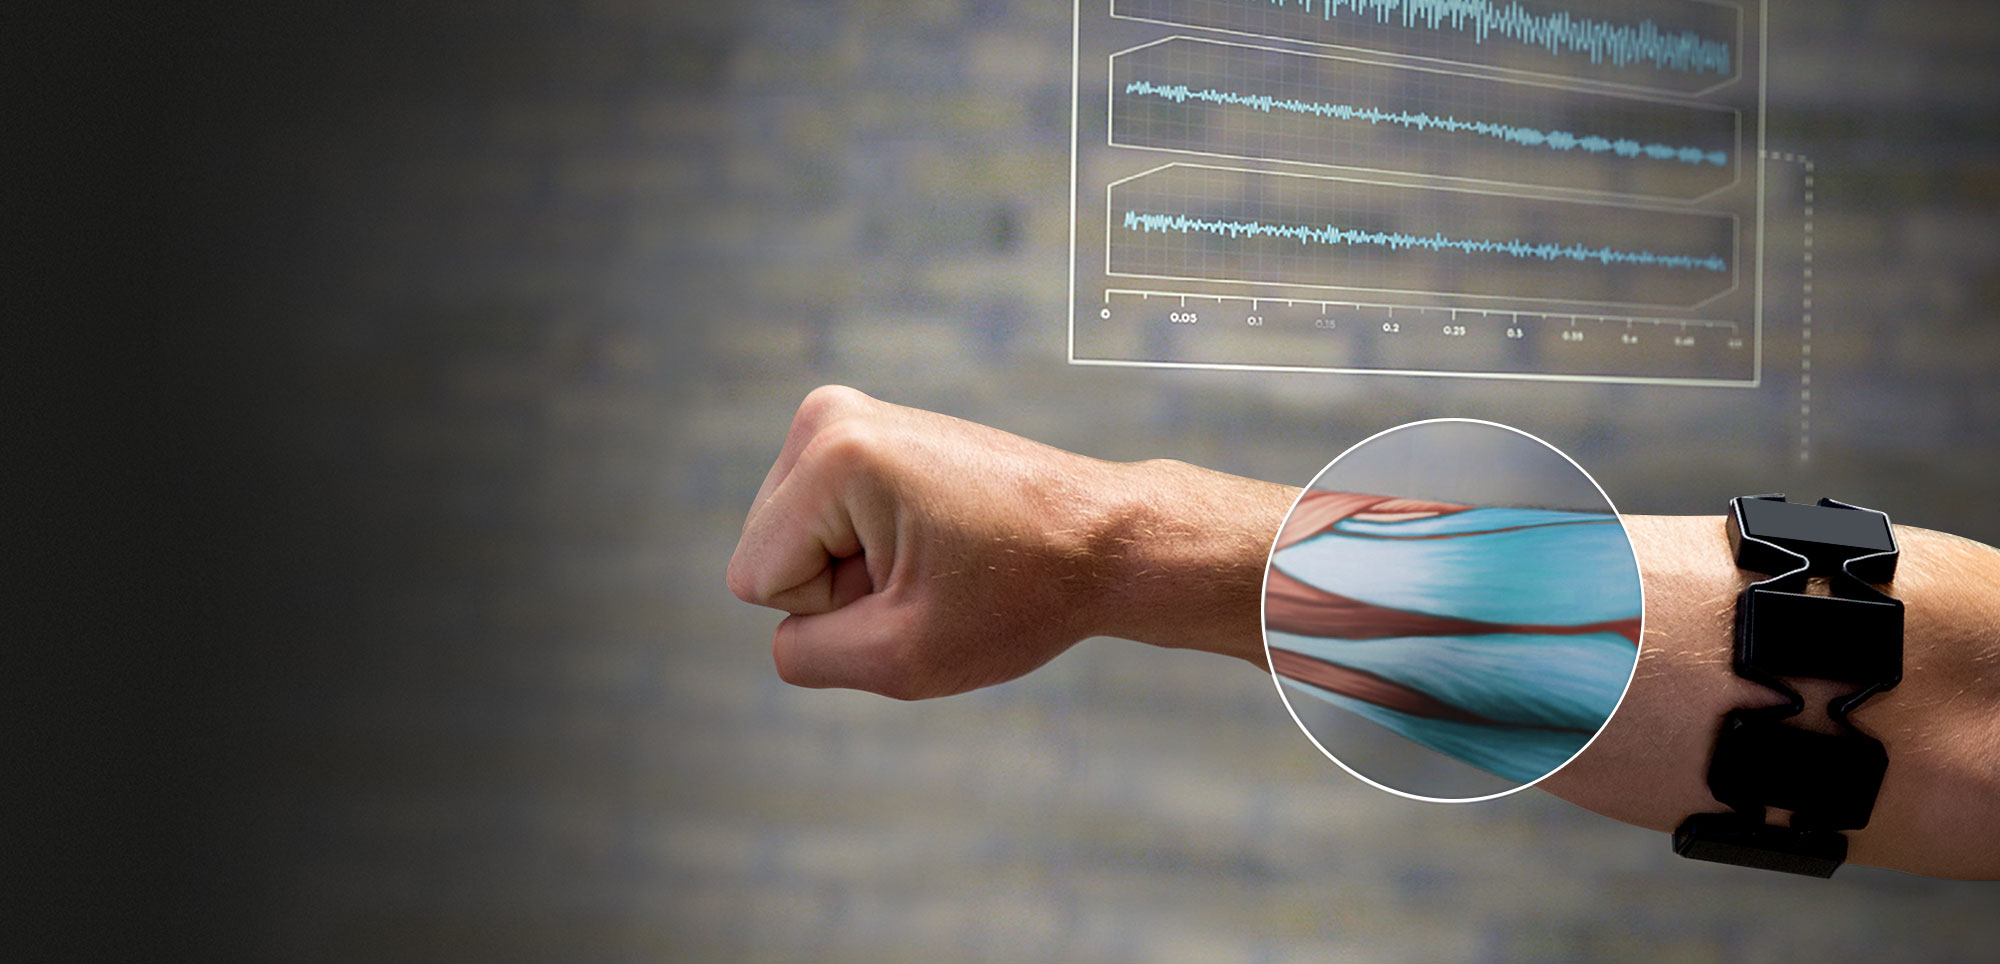
\includegraphics[width=\linewidth]{pictures/myo_armband.jpg}
	\caption[The Myo armband]{The Myo armband is a gesture recognition device worn on the forearm and manufactured by Thalmic Labs. 
	The Myo enables the user to control technology wirelessly using various hand motions. 
	It uses a set of electromyographic (EMG) sensors that sense electrical activity in the forearm muscles, combined with a gyroscope, 
	accelerometer and magnetometer to recognize gestures~\citep{Myo2015}.}
	\label{fig:myo}
\end{figure}

\paragraph{Vision-based devices} usually make use of either depth-aware cameras or stereo cameras to approximate a 3D representation of what's output by the cameras, 
which in many ways are similar to how the human eyes work. 
Products making use of this technology include the Microsoft's Kinect and the Leap Motion controller (see figure \ref{fig:leapmotion}). 

\begin{figure}%[h!] %[H]
	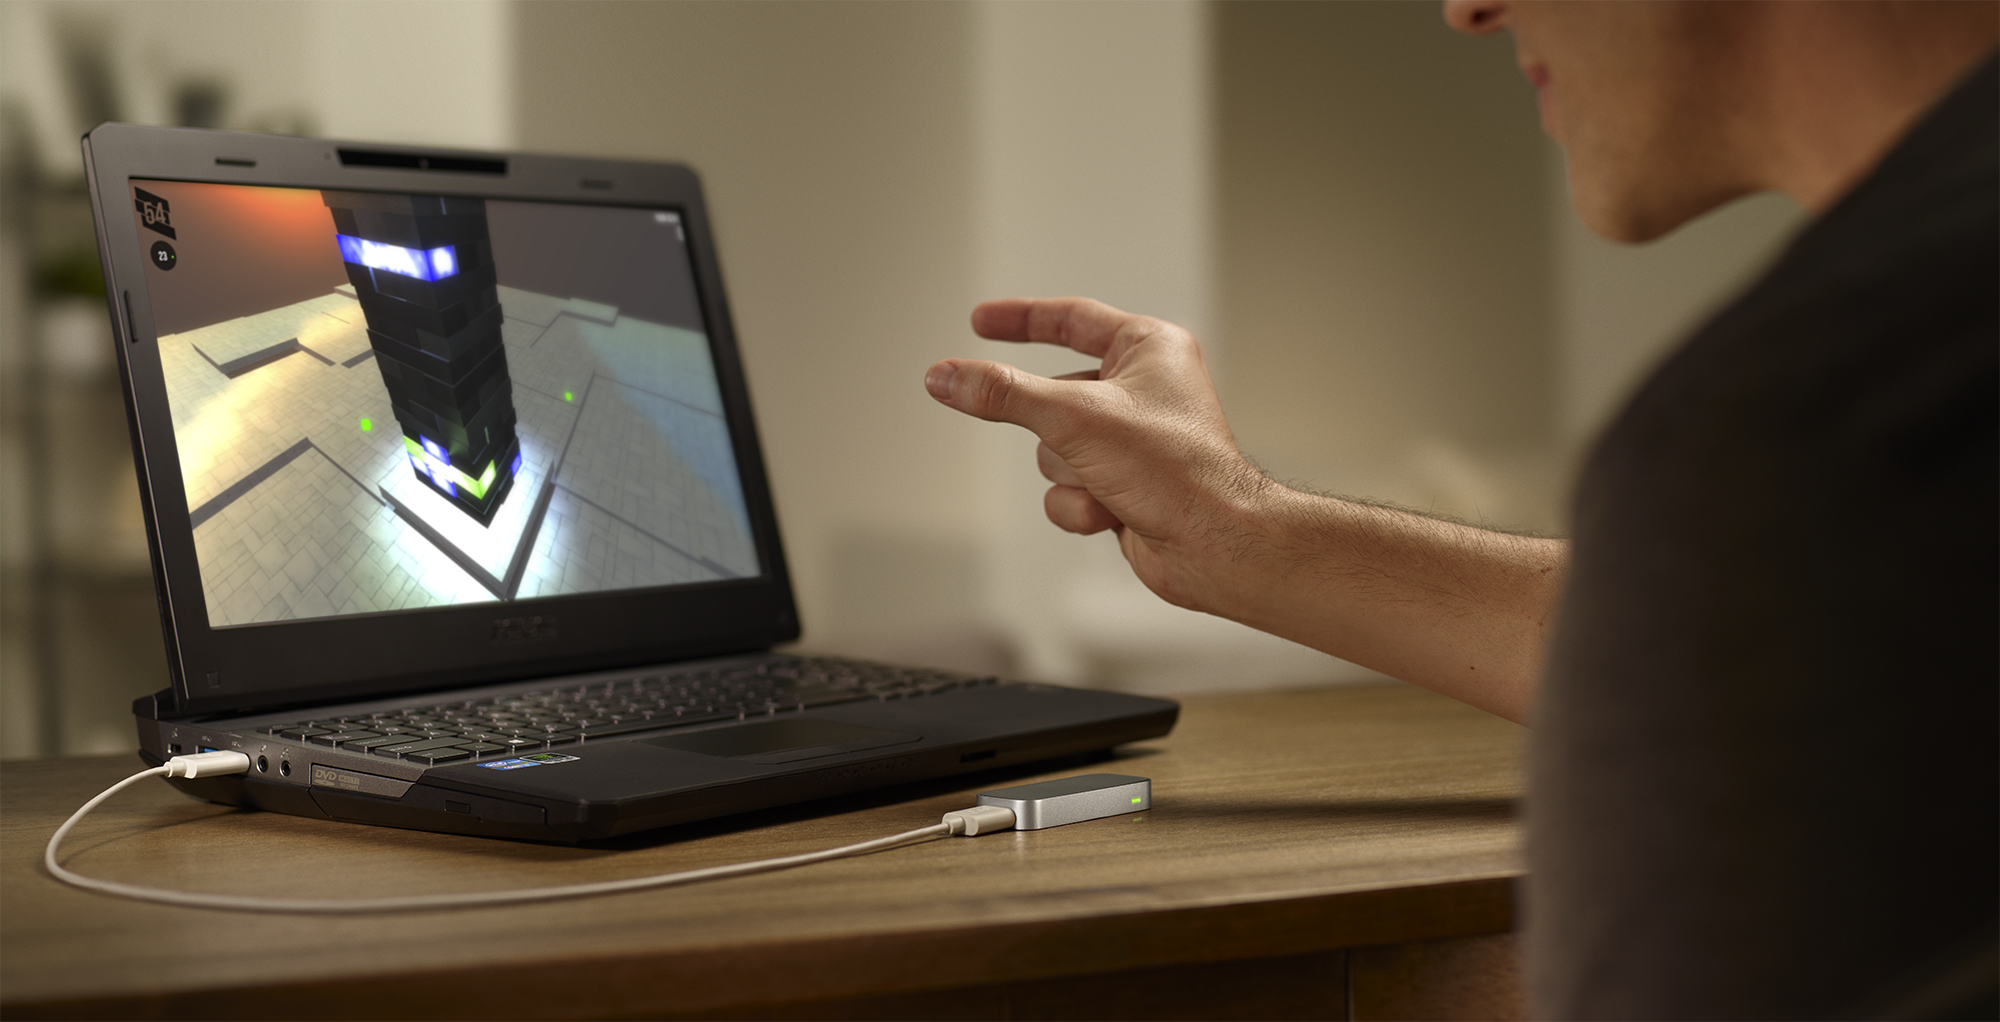
\includegraphics[width=\linewidth]{pictures/leapmotion2.png}
	\caption[The Leap Motion Controller]{The Leap Motion Controller is a small USB peripheral device which is designed to be placed on a physical desktop, 
	facing upward. Using two monochromatic IR cameras and three infrared LEDs, the device observes a roughly hemispherical area, to a distance of about 1 meter, 
	and generates almost 200 frames per second of reflected data~\citep{LeapMotion2016}.}
	\label{fig:leapmotion}
\end{figure} 

\paragraph{}Both approaches have their advantages and disadvantages (see~\citet{Rautaray2015} for a deeper discussion of these). 
Contact-based devices generally have a higher accuracy of recognition and a lower complexity of implementation than that of vision-based ones. 
Vision-based devices are on the other hand seen as more user friendly as they require no physical contact with the user. 

The main disadvantage of contact-based devices is the potential health hazards, which may be caused by some of its components~\citep{Schultz2003}. 
Research has suggested that mechanical sensor materials may raise symptoms of allergy and magnetic component may raise the risk of cancer~\citep{Nishikawa2003}. 
Even though vision-based devices have the initial challenge of complex configuration and implementations, 
they are still considered more user friendly and hence more suited for usage in long run. Because of the reasons outlined above this thesis will primarily 
be oriented towards vision-based gesture recognition technologies. 

\subsection{The primary Vision-based Technologies}
Today, there are three primary vision-based technologies that can acquire 3D images: Stereoscopic vision, structured light pattern and time of flight (TOF)~\citep{Ko2012}.
These all make use of one or several cameras and lights to capture and recognize certain movements or poses from the user, and transform it to a certain action on the computer (e.g.~a recognized finger tap might be the equivalent to left mouse button click). 

\paragraph{Stereoscopic vision}is the most common 3D acquisition method and uses two cameras to obtain a left and right stereo image. These images are slightly offset on the same axis as the human eyes. As the computer compares the two images, it develops a disparity image that relates the displacement of objects in the images.

\paragraph{Structured light pattern}measure or scan 3D objects through illumination. Light patterns are created using either a projection of lasers or LED light interference or a series of projected images. By
replacing one of the sensors of a stereoscopic vision system with a light source, structured-light-based technology basically exploits the same triangulation as a stereoscopic system does to acquire the 3D coordinates of the object. Single 2D camera systems with an IR- or RGB-based sensor can be used to measure the displacement of any single stripe of visible or IR light, and then the coordinates can be obtained through software analysis.

\paragraph{Time of flight}is a relatively new technique among depth information systems
and is a type of light detection and ranging (LIDAR) system that transmits a light pulse from an emitter to an object. A receiver determines the distance of the measured object by calculating the travel time of the light pulse from the emitter to the object and back to the receiver in a pixel format.

\begin{figure}%[h!] %[H]
	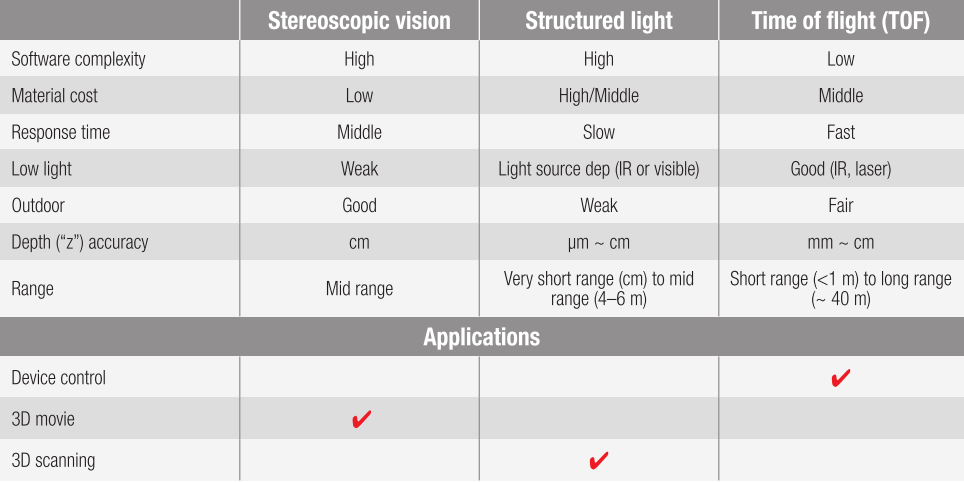
\includegraphics[width=\linewidth]{pictures/Vision-based_comparisons.png}
	\caption{Comparison of Vision-based sensor technologies~\citep{Ko2012}.}
	\label{fig:VBComparisions}
\end{figure} 

\paragraph{Of these technologies} stereoscopic vision is perhaps the most promising one for the consumer market as it has the lowest material cost~\citep{Ko2012}, and has proved more reliable in variable light conditions than its counterparts. One of the latest consumer-oriented devices of this kind is the Leap Motion Controller, which distinguishes itself for having a higher localization precision than other depth vision-based devices~\citep{Weichert2013}, and also for capturing depth data related to palm direction, fingertips positions, palm center position, and other relevant points~\citep{Wei2016}. The Leap Motion Controller will be reviewed more in-depth in the next section. 

\subsection{How vision-based devices functions}


\section{Gesture Recognition Principles}
A gesture can be defined as a physical movement of the hands, arms, face and body with the intent to convey information or meaning~\citep{Mitra2007}, 
Even though the use of keyboard and mouse is a prominent interaction method, there are situations in which
these devices are impractical for human-computer interaction (HCI). This is particularly the case for interaction with 3D objects~\citep{Rautaray2015}. 

To be able to convey semantically meaningful commands through the use of gestures one must rely on a gesture recognition system, 
which is responsible for capturing and interpreting gestures from the user and, if applicable, carry out the desired action. 
Often this process is seen as a sum of three fundamental phases: Detection, tracking and recognition~\citep{Rautaray2015}.
This section will describe what makes up a gesture recogntion system.

\subsection{Detection}
The first step in a typical gesture recognition system is to detect the relevant parts of the captured image and segment them from the rest. 
This segmentation is crucial because it isolates the relevant parts of the image from the background to ensure that only the relevant part is processed by the subsequent 
tracking and recognition stages~\citep{Cote2006}. 
A gesture recognition system will typically be interested in hand gestures, head- and arm movements and body poses, and thus only these factors should be observed by the system.

\subsection{Tracking}
The second step in a gesture recognition system is to track the movements of the relevant segments of the frames, e.g.~the hands. 
Tracking can be described as the frame-to-frame correspondence of the segmented hand regions and aims to understand the observed hand movements. 
This is often a difficult task as hands can move very fast and their appearance can change vastly within a few frames, 
especially when light condition is a big factor~\citep{Wang2010}. 
One additional note is that if the detection method used is fast enough to operate at image acquisition frame rate, it can also be used for tracking~\citep{Rautaray2015}.   

\subsection{Recognition}
The last step of a gesture recognition system is to detect when a gesture occurs. 
This often implies checking against a predefined set of gestures, each entailing a specific action. 
To detect static gestures (i.e postures involving no movement) a general classifier or template-matcher can be used, 
but with dynamic gestures (which involves movement) other methods, which keep the temporal aspect, such as a Hidden Markov Model (HMM), are often required~\citep{Benton1995}. 
The recognition technology often makes uses of several methods from the field of machine learning, including supervised, unsupervised and reinforced learning.

When a gesture recognition system detects a relevant segment, it is thus tracked and represented in some way in the system. For hand gesture representations, 
which is the most relevant for this thesis, there are two major categories of hand gesture representations: 3D model-based methods and appearance-based methods~\citep{Rautaray2015}.

\begin{figure}%[h!] %[H]
	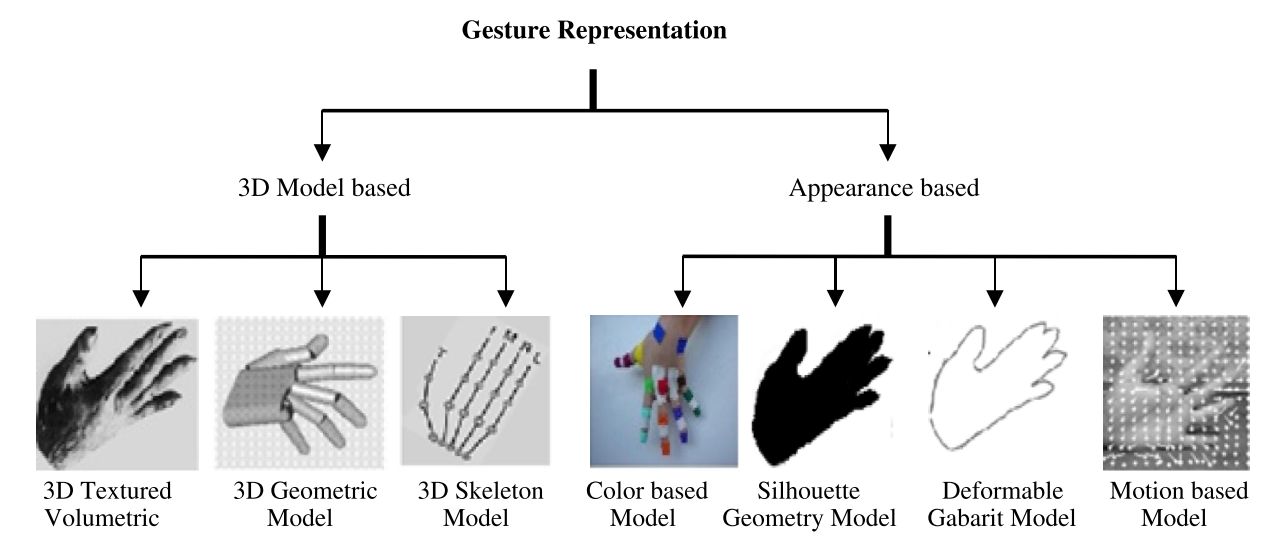
\includegraphics[width=\linewidth]{pictures/gesture_representation.png}
	\caption[Vision-based hand gesture representations]{Vision-based hand gesture representations~\citep{Bourke2007} }
	\label{fig:oculus}
\end{figure}


\section{Challenges with VR and GRT} 
Problems with using VR + e.g Leap over mouse + keyboard + display. E.g:

\subsection{The "writing issue"}
Virtual keyboards are bad. 
Regular keyboards are impractical. 
See "ideer til masteroppgaven.txt"

\subsection{Challenges in "designing" gesture schemes}
People have different preferences. Have intuitive gestures. Have gestures that is not too
fatiguing. Have gesture with high precision and recall (F-score) (high TP and TN. Low FP, FN).
Have a system that doesnt mistake one gesture for another.

\subsubsection{Fixes?}
User-gesture calibration. 

\section{Related work}


% Creation and implementation of such efficient and
% accurate hand gesture recognition systems is aided by two major types of enabling
% technologies for human-computer interaction, namely contact-based and vision-based devices~\citep{Rautaray2015}. 